\documentclass[12pt,a4paper,twoside]{report}

\usepackage[lmargin=2.54cm,tmargin=2.54cm,rmargin=2.54cm,bmargin=2.52cm]{geometry}
\usepackage[utf8]{inputenc}
\usepackage[T1]{fontenc}

\usepackage{mathptmx}
\usepackage{fancyhdr}
\usepackage{graphicx}
\usepackage{subcaption}
\usepackage{pdfpages} 
\usepackage{amsmath}
%\usepackage{showframe}

\pagestyle{fancy}
\fancyhf{}
\fancyhead[LE,RO]{Interim Report}
\fancyhead[RE,LO]{Akinola Alexander Dada}
\fancyfoot[CE,CO]{\leftmark}
\fancyfoot[LE,RO]{\thepage}

\linespread{1.5}

\title{Interim Report \\ Dynamic Modelling, Simulation and Control of Asymmetrical VTOL Multi-Rotor UAVs}
\author{Akinola Alexander Dada \\ 160140802}
\date{$\today$}

\begin{document}
		
	\maketitle
	\newpage
	\section*{\underline{Project Background}}
	 
		Unmanned Aerial Vehicle (UAV) are aerial systems which are not directly controlled by a human onboard the vehicle. There are many types of UAV platforms chiefly defined by the characteristics of their mechanical constructions, such as the on frame position, number and type of their actuators. One such type of UAVs are multi-rotors which are defined as such due to their multiple rotor wing actuators [5],[6]. 
		\\
		These types of UAVs have a wide range of applications due to their ability to perform vertical take-off and landing (VTOL), stationary and low speed flight [5], coupled with their relatively simple mechanical designs when compared to single rotor constructions, such as more traditional helicopters [2]. These features enable them to be utilised in many wide ranging applications, where it would not be possible to use other platforms, such as; large scale directed administration of substances to plants in precision agriculture, frequent inspection of standing structures, wide area surveillance, amongst many others [10],[11].
		\\
		The major challenge in dealing with these types of UAVs is their inherent instability in flight, save for the intervention of complex control systems [1],[2],[3],[4],[5]. For this reason, control schemes must be implemented in order for multi-rotor UAVs to be utilised. Therefore in order to ensure control schemes meet performance specifications in an energy efficient manner, it is necessary to understand the physical characteristics and response to stimuli of the system which is done through mathematical modelling. This level of insight is also required in the development of many advanced control schemes. [11],[14].
		
	\section*{\underline{Aims and Objectives}}
		
		The framework of this project is set around the design and development of control software for Vertical/Short Take-off and Landing (VSTOL) model aircraft. From this theme, the aims of modelling and simulating the non-linear dynamics of an asymmetrical VTOL multi-rotor platform and the development of multiple control schemes were derived. These control schemes will then be implemented on the multi-rotor platform via an embedded microprocessor unit. 
		\\
		These aims breaks down in to multiple objective milestones which must each be achieved to fulfil the full scope of that the aim outlines. These Objectives can be Classified into 2 categories:

			\subsection*{Basic Objectives}
			
				\begin{enumerate}
					\item
						Develop a mathematical model representing the dynamics of the multi-rotor aircraft.
					\item
						Develop a dynamic simulation of the crafts behaviour.
					\item
						Develop feedback control laws: Proportional Integral Derivative(PID) and Linear Quadratic Gaussian(LQG).
					\item
						Investigate feedback control laws in simulation with the mathematical model to achieve behavioural targets.
					\item
						Develop flight control software to interface with sensors and implement control laws.
					\item
						Implement the flight control software on an embedded microprocessor unit.
					\item
						Implement controller unto multi-rotor platform.
					\item
						Discuss the results of performance comparisons between the simulation and hardware implementations.
				\end{enumerate}
			
			\subsection*{Advanced Objectives}
			
				\begin{enumerate}
					\item
						Investigate the application of Model Predictive Control(MPC) schemes in simulation.
					\item	
						Incorporate and implement MPC schemes unto the flight control software.
					\item	
						Discuss the differences between the PID, LQG and MPC implementations.
				\end{enumerate}
		
	\section*{\underline{Review of Literature and Work Till Date}}
		
		The acquired literature take the form of articles published in scientific journals, Research publications, exerts from university Lectures, Masters and PhD thesis publications and published books, which present 3 major themes that are relevant to the project's investigation:
		
		\begin{itemize}
			\item 
				Mathematical Modelling and Systems Identification.
			\item
				Control Design.
			\item
				Simulation and Implementation.
		\end{itemize}
				
		\section*{UAV}
			\begin{figure}[h!]
				\centering
				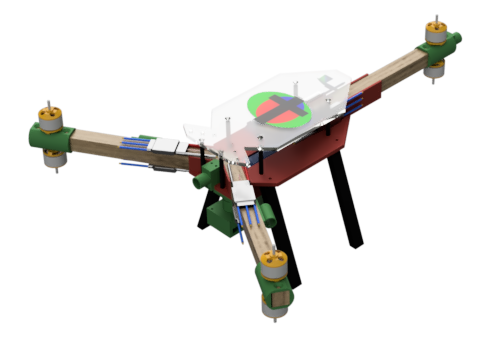
\includegraphics[width=0.6\linewidth]{Y6_Hexarotor2.png}
				\caption{Y6 Hexarotor CAD Graphic}
				\label{fig:Y6Hexarotor}
			\end{figure} 
		
			The selected UAV under consideration is one of my own design, which is an asymmetrical Y6 Hexarotor, meaning that its has 6 actuators which are arranged in such a configuration where it resembles the shape of  a "Y". This kind of configuration has its actuators is 3 coaxial pairs, meaning two motors one atop the other back to back, which has the advantage of minimising the size of the frame while enabling higher thrust and stability. However there are added power demands and inefficiency due to the increased number of actuators and the aerodynamic interaction of coaxial actuator combinations [6].
			\\
			The UAV is actuated by 6 1000Kv brushless direct current (BLDC) motors attached to 6 10x45inch propellers and is powered by a 4-cell lithium-polymer battery with an operational voltage range of 16.8 volts to 12.8 volts. The UAV has dimensions of, 45 cm in length from rear motor centres to from motor centres, 44 cm in length from left motor centres to right motor centres, and a mass of 2.1 kilograms. control systems will be implemented on a BeagleBone Blue linux based single board computer (SBC).
			\\
			The exact details involved with the design, development and construction of UAVs is beyond the scope of the project investigation but are fully explored in [19].
		  
		\section*{Mathematical Modelling and System Identification}
		
			\subsection*{Rigid-Body Dynamics}
			
				In modelling, it is necessary to state assumptions made about its characteristics. Multi-rotors can be  defined as a rigid body free to move within 3D space. Therefore it moves with 6 degrees of freedom (6-DOF). With this modelling assumption,  the motion of the vehicle is subject to the laws of rigid body Kinematics and Kinetics. Vehicle motion is defined in terms of 2 coordinate frames moving relative to one another where the physical quantities that change with time, its states, change with respect to one frame or the other. They are; Earth Frame: \(Fe\), Attached to the earth, Body Frame: \(Fb\), Attached to the vehicle body. Each frame consists of 3 orthogonal axes, \(xE yE zE\) and \(zB yB zB\) respectively about which rotational motion can occur, and along which translational motion can occur [1],[2],[3],[4].
				\\
				The sources obtained explore 2 ways for representing rotational motion. Euler angles are used to describe arbitrary orientation in the 3-dimensional Euclidean space, three parameters are required. Euler angles represent a sequence of three elemental rotations about each axes of a coordinate system. Any orientation in 3D space can be achieved by composing these 3 elemental rotations [2],[4]. Another representation is through Quaternions which solve issues present with computing Euler angles such as computational expense and rotational singularities which occur when during certain orientations, as it does not require the calculation of $\sin$ and $\cos$ when certain angles go to 0 or 90 degrees and their multiples. Quaternions represent orientation using a single angle about an axis [4],[14].
				\\ 
				The rigid body assumptions also allows for the utilisation of several Mechanical Modelling techniques and conventions which are used to derive the non-linear dynamics of mechanical systems taking into account both kinematics and Kinetics:
				
				\begin{itemize}
					\item 
						The Newton-Euler. [1],[2],[3],[4],[5],[10],[13],[14],[15],[16]
					\item
						The Euler-Lagrange. [4],[16]
					\item
						The Newton-Hamiltonian.
					\item 
						Hardware-in-Loop system identification. [11]
				\end{itemize}
				
				This investigation utilises both the Euler-angle representation and the Newton-Euler convention due to its intuitively familiar representation of systems dynamics from the first principles of newtons 2nd law showing the effects of forces applied to the rigid body by its actuators.
				\\
				Due to the UAVs Layout, it is asymmetric, this creates a system where inertia is not represented by a diagonal matrix but instead one with off diagonal elements and transposed reference frames [7],[8]. However, for the purpose of this investigation, it is assumed that the system is symmetrical as the off diagonal terms in the inertia matrix are far lower in magnitude than the diagonal terms, thus can be reasonably neglected. Otherwise, the entire coordinates system would be adjusted and transformed to produce a true diagonal matrix as presented in [8].
				\\
				In order to design the controllers, the non-linear model obtained via the Newton-Euler convention needs to be linearised. This is accomplished through the application of Jacobi's linearisation as presented in [12]. This process produces a full linear state space representation of systems dynamics around stable operating points. 
				
			\subsection*{Actuator Dynamics}
			
				As stated in the \emph{UAV} section, the multi-rotor is actuated by BLDC motors. To fully develop a system model, these must be modelled. This can either be done via first principles calculations as in [2],[3],[16] or via experimental systems identifications as presented in [4],[6],[9],[10],[11],[14],[17]. This approaches involves the derivation of a lumped parameter linear input output model, encompassing the electronic speed control, motor and propeller dynamics, between input Pulse width modulated (PWM) signal duty cycles or pulse width and the output angular velocities torque and thrust forces. This has the advantage of reducing complex dynamics enabling the utilisation of a minimum viable model and as such is being implemented in this investigation.Once the actuator dynamics are identified they will substitute the dummy place holder values taken from data presented in [14].
			
			\subsection*{Results}
			
				Presentation of the system's non-linear dynamics.
				\\
				In the Body frame:
				\[I\nu' = \tau - \nu X (I\nu)\]
				
				$$
				I
				\begin{bmatrix}
				p'\\
				q'\\
				r'\\
				\end{bmatrix}
				=
				\begin{bmatrix}
				\tau_\phi\\
				\tau_\theta\\
				\tau_\psi\\
				\end{bmatrix}
				-
				\begin{bmatrix}
				p\\
				q\\
				r\\
				\end{bmatrix}
				(X)
				I
				\begin{bmatrix}
				p\\
				q \\
				r\\
				\end{bmatrix}
				$$
				\\
				Where \(p, q, r, p', q', r'\) are angular velocities and accelerations, I is the diagonal inertia matrix and $\tau$ is a vector of the torques generated form the actuators and UAV body.
				\\
				In the Earth frame:
				\[M \zeta'' = G + RT_b - D\zeta' \]
				
				$$
				M
				\begin{bmatrix}
				 x''\\
				 y''\\
				 z''\\
				\end{bmatrix}
				=
				-Mg
				\begin{bmatrix}
				0\\
				0\\
				1\\
				\end{bmatrix}
				+
				T_b
				\begin{bmatrix}
				C\phi S\theta C\psi + S\psi S\phi \\
				C\phi S\theta S\psi - S\phi C\psi \\
				C\phi C\theta \\
				\end{bmatrix}
				-
				D
				\begin{bmatrix}
				x'\\
				y'\\
				z'\\
				\end{bmatrix}
				$$
				\\
				Where M is mass, \(x, y, z, x',y',z',x'', y'', z''\)  are linear position, velocity and acceleration,\(\phi,\theta, \psi\) are Euler angles, D is the diagonal matrix of air resistance and $T_b$ is a vector of the Forces generated form the actuators. This was then turned into a Simulink Function block:
				
				\begin{figure}[h!]
					\centering
					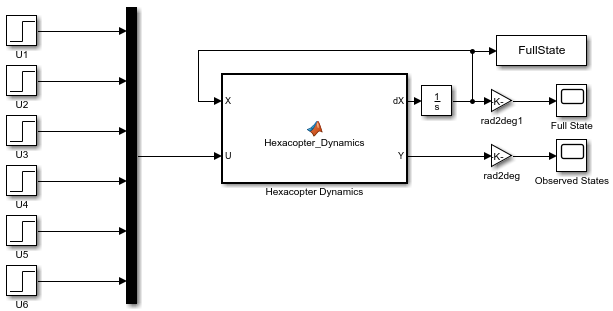
\includegraphics[width=0.8\linewidth]{sim.png}
					\caption{Non Linear Dynamics in Simulink}
					\label{fig:Sim}
				\end{figure} 
				 
				
		\section*{Control Design simulation and Implementation}
			
			The three control schemes under investigation are: 

			\subsection*{PID}
			
				PID controllers consist of a component proportional to the error between a desired value and the observed value, a component proportional to the derivative of the error, and on which is proportional to the integral of the error. Adding an integral term causes any remaining steady-state error to build up and enact a change on the input signal to the system, so a PID controller should be able to track target trajectories with small to zero steady-state error.[3] In practical implementations, pure PID controllers come with drawbacks like integral wind-up and derivative noise sensitivity which  must be dealt with during the implementation stage[21]. Another issue is, PID contollers are designed for Single input and output systems thus any implementation for a multiple input and output system like a UAV will not take into account dynamic coupling between states. [14] presents an novel way to overcome this by designing the PID controller using LQG techniques.
				
			\subsection*{LQG}
			
				The Linear Quadratic Gaussian makes use of the full state of a system through the application of a Gaussian estimator, in this case a Kalman filter, to obtain the full state. It is a form of optimal control where its objective is to minimize a cost or performance function to bring the system’s state to a desired set of values while minimizing the use of the control inputs[2][14][20][21]. As of the creation of this report, significant work has been done ahead of schedule in beginning the development an LQG controller. Below is the MATLAB Simulink simulation showing the an LQG control structure in series with the multi-rotor dynamics.
				
				\begin{figure}[h!]
					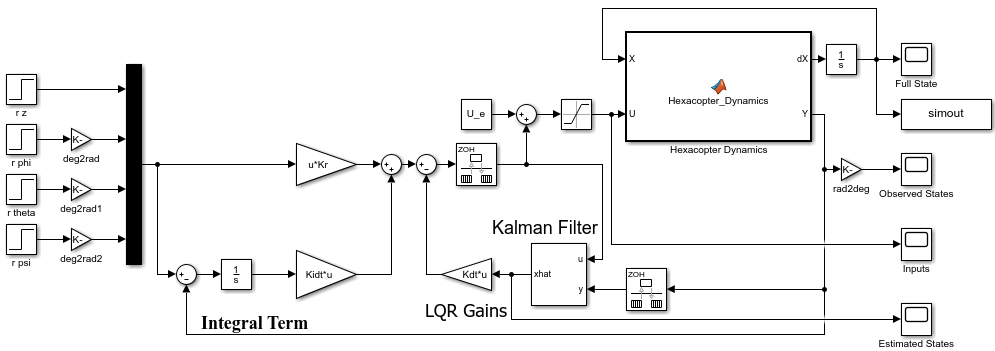
\includegraphics[width=\linewidth]{LQGsim.png}
					\caption{Dynamics and LQG controller in Simulink}
					\label{fig:LQGsim}
				\end{figure} 
			
			\subsection*{MPC}
				Like LQG, MPC is also a kind of optimal control, however, this technique's cost function includes the values of future states over some fixed finite horizon and control signals can be determined so that the system can meet physical constraints. MPC is also known as receding horizon control(RHC) as when it only acts on the first step in the horizon of states before recalculating and performing this action until the target is achieved[11]. The LQG can be referred to as an infinite horizon controller as it does not recede the horizon[18].
				\\
				Study [11] also discuses various implementations methods including utilising machine leaning techniques to estimate certain optimisation parameters, as well as proposing and implementing such a controller.
		
		\section*{Summary}
		
			Thus far, the assembly of the multi-rotor platform, displayed in the \emph{UAV} section, has been completed with all the parts of the frame including the actuators and propellers present, access to pertinent literature concerning; the mathematical modelling of rigid bodies, the system identification of actuator dynamics, the design and implementation of a myriad of linear and non-linear state feedback techniques, as well as to those beginning investigations into the more advanced topic of model based predictive control, have been obtained. 
			\\
			In working towards the objectives layed out in the \emph{Aims and Objectives} section,  the full non-linear mathematical model of the rigid body dynamics of the multi-rotor platform have been developed and implemented as a simulation in MATLAB/Simulink, as well as Linear State Space representations of the system for the purposes of control design, with work having commenced on the design of an LQG controller
			\\
			
	\newpage
		
	\section*{\underline{Project Management}}
	
		In accordance with the project \emph{Aims and Objectives}, significant progress has been made particularly towards the timeous completions of \emph{Basic Objectives} points 1, 2, 3 and 4 which will be due for completion and review in accordance with the project plan. Thus far, the project has proceeded on schedule, therefore no changes have been made to the plan submitted on week 6. Purchases have been made acquiring key hardware such as the main flight computer, the radio control system, which will serve as the main communication unit sending control commands to the multi-rotor. Orders have also been put in for the more motors, electronics speed controllers, and load cells which will be used to develop the lab-bench platforms that will serve to identify the actuator dynamics specified in the \emph{Actuator Dynamics} section. Future completion dates for further objectives are displayed in the project plan expressed in the table below with the in the full project Gantt chart available in the \emph{Appendix}.
		\\  
		
		\begin{figure}[b]
			\centering 
			\caption{Table of Project Objectives and Dates}
			\label{fig:Project Objectives and Dates}
			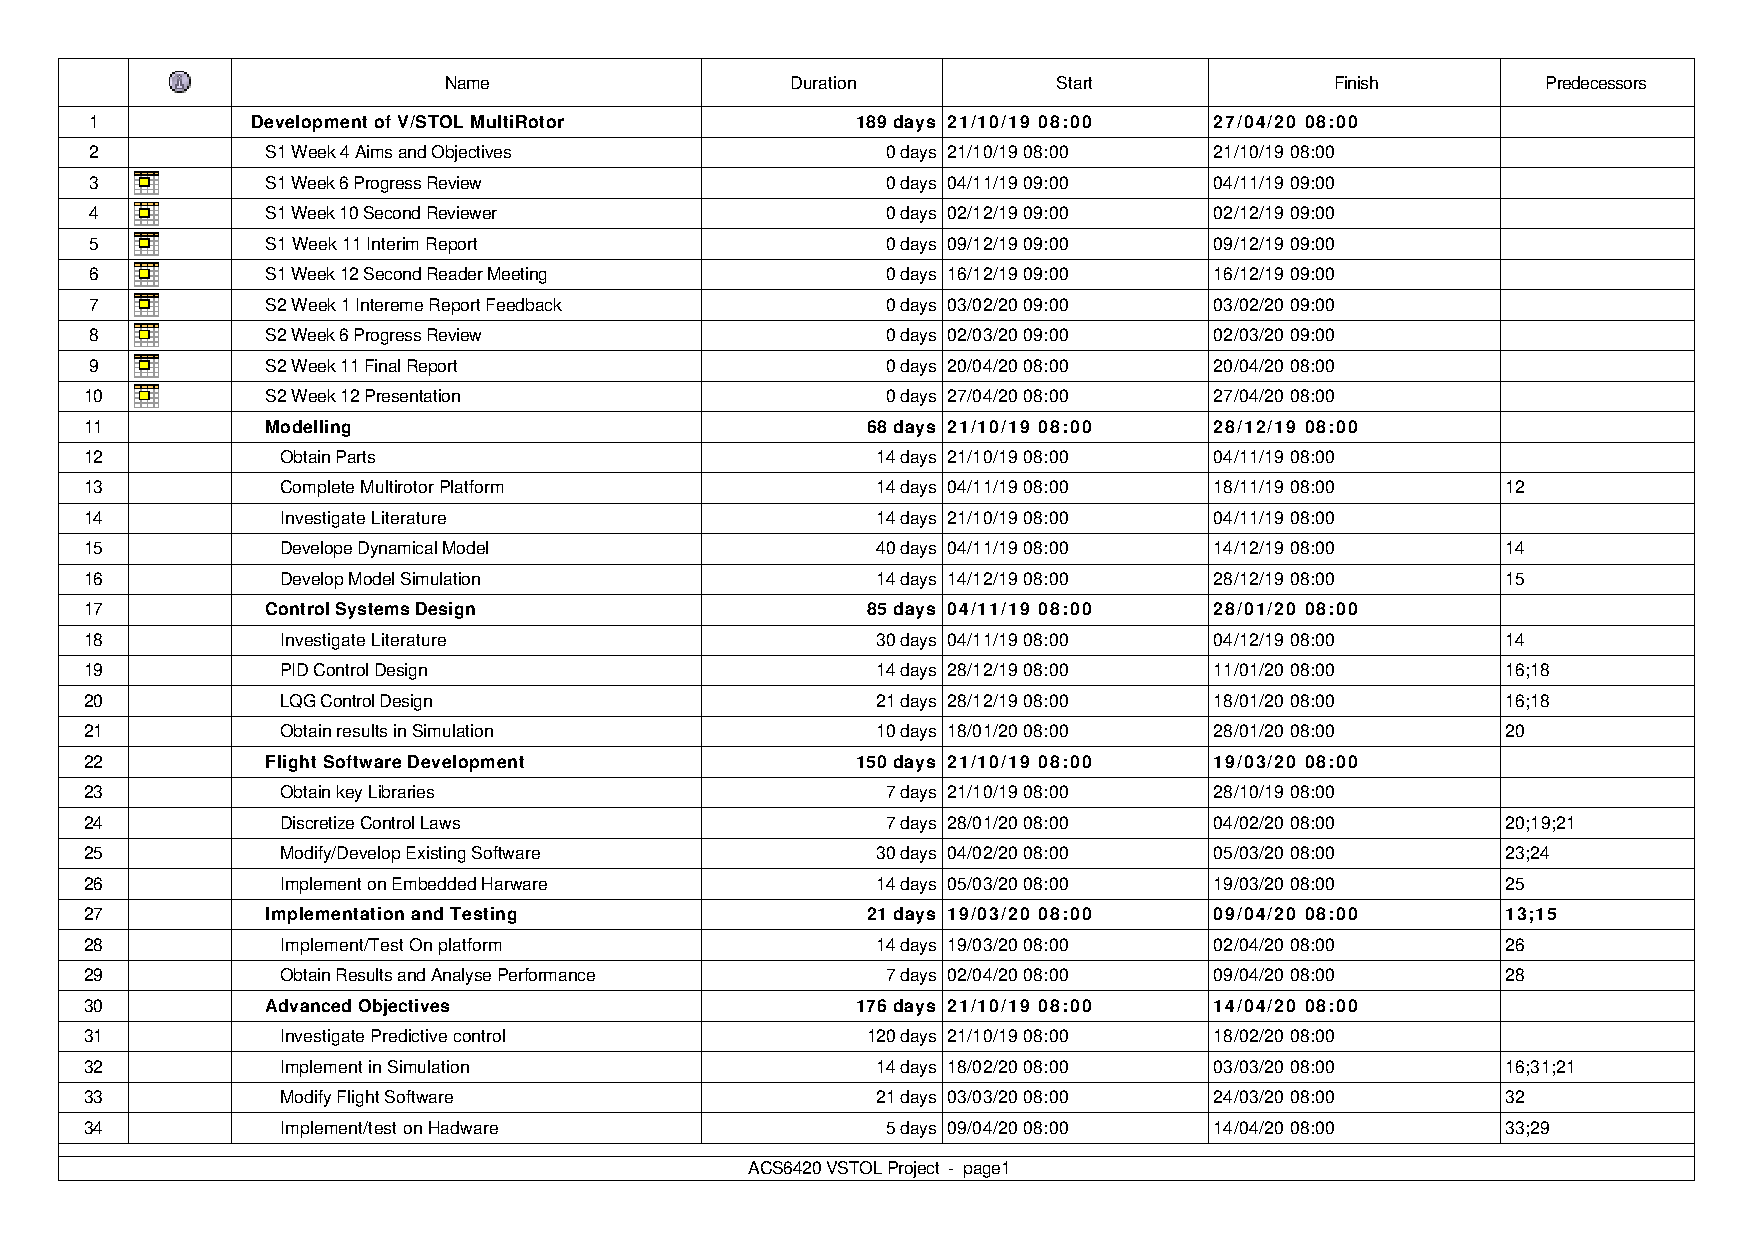
\includepdf[pages=1,pagecommand={},offset=0cm -4.75cm]{Gantt}
		\end{figure}
	
	\newpage
	
	\section*{\underline{Self Review}}
		
		In dealing with project operations, there have been several challenges most prominently those involved with obtaining and simulating the multi-rotor's dynamics. The work done in understanding the complex mechanics, which is one of my weakest subjects, has been very helpful in gaining insight into the workings of dynamical systems at large. Proving to be a task of decent difficulty is learning how to utilise the full range of capabilities provided by Matlab/Simulink. This is displayed by the fact that the rigid body simulation the presented in the \emph{Results} section breaks down due to singularities forming, the issue raised in the \emph{Rigid-Body Dynamics} section. I am yet to fully diagnose the issue, most likely this is due still no fully understanding how to represent a simulation of such complex dynamics.
		\\	   
		I have had to balance work on this projects with other modules which has been challenging. Though, at the time of creating this report, work has progressed on time and on-schedule towards achieving the first 4 objectives listed in the \emph{Basic Objectives} section. This has been a great exercise in developing the ability to manage a project not only in the scope of the project across time with setting achievable objectives, as the scope of the project has been revised down from designing control systems for a full Quad-Tilt multi-rotor, to where it is now.  but also in managing individual activities such as parts purchasing.
		
		
	\newpage
	%\renewcommand{\bibname}{\underline{References}}
	
	\begin{thebibliography}{20}

		%\addcontentsline{toc}{section}{References}
		
		\bibitem{MODELLINGZoranBenic}Zoran Benic, Petar Piljek, Denis Kotarski. Interdisciplinary Description of Complex Systems 14(1), 88-100 Mathematical Modelling Of Unmanned Aerial Vehicles With Four Rotors. (2016)
		
		\bibitem{ThesisFrancescoSabatino}Francesco Sabatino. KTH Electrical Engineering, Master's Thesis: Quadrotor Control, Modeling, Non-linear Control design, and Simulation. (2015)
		
		\bibitem{QuadrotorDynamics}*author unknown*. Quadcopter Dynamics, Simulation, and Control.
		
		\bibitem{ParameterIdentificationSurveyAnzekaChovancova}Anzeka Chovancova, Tomas Fico, Lubos Chovenec, Peter Hubinsky. Procedia Engineering 96, 172-181. Mathematical Modelling and Parameter Identification of Quadrotor (a Survey). (2014)
	
		\bibitem{ModellingDenisKotarskiDenisKotarski}Denis Kotarski, Petar Piljek, Matia Krznar. International Journal of Theoretical and Applied Mechanics. Mathematical Modelling of Multirotor UAV. (2016)
		
		\bibitem{DevelopmentOfCoAxialY6RomanCzyba}Roman Czyba, Grzegorz Szafranski, Marcin Janik, Krzysztof Pampuch, Michal Hecel. International Conference on Unmanned Aircraft Systems (ICUAS) Denver Marriott Tech Center Denver, Colorado, USA. Development of Co Axial Y6 Rotor UAV  Design, Mathematical Modelling, Rapid Prototyping and Experimental Validation. (2015)
		
		\bibitem{RigidBodyDynamicsUTAHSTATE}Utah State Uinversity, Classical Mechanics- Rigid Body Dynamics. (2012)
		
		\bibitem{RigidBodyDynamicsMITJ.Peraire}J. Peraire, S. Widnall, Massatusettes Institute of Technology, 16.07 Dynamics Version 2.1. Lecture L26 - 3D Rigid Body Dynamics: The Inertia Tensor. (2008)
		
		\bibitem{PropulsionSystemCharacterizationGautierHattenberger}Gautier Hattenberger, Antoine Drouin, Murat Bronz. University of Toulouse ENAC F-31077 Toulouse, France. Electric Propulsion System Characterization through Experiments. (2018)
		
		\bibitem{ThesisPieroGrazianoIoppo}Piero Graziano Ioppo. Department of Electrical and Electronic Engineering: Stellenbosch University, Master's Thesis: The Design, Modelling and Control of an Autonomous Tethered Multirotor UAV.(2017)
		
		\bibitem{On-boardMPCPatrickBouffard}Patrick Bouffard. Electrical Engineering and Computer Sciences University of California at Berkeley, Technical Report No. UCB/EECS-2012-241, http://www.eecs.berkeley.edu/Pubs/TechRpts/2012/EECS-2012-241.html. 
		On-board Model Predictive Control of a Quadrotor Helicopter: Design, Implementation, and Experiments.(2012)
		
     	\bibitem{LinearizationAndrewPackard}Andrew Packard. California Institute of Technology. Dynamic Systems and Feedback-19, Jacobian Linearizations, equilibrium points. (2002)
     	
		\bibitem{ThesisHaoquanYe}Haoquane Ye. Department of Electrical Engineering and Computer Science CASE WESTERN RESERVE UNIVERSITY, Master's Thesis: CONTROL OF QUADCOPTER UAV BY NONLINEAR FEEDBACK. (2018)
		
		\bibitem{LQR/LQGRafaelGuardeno}Rafael Guardeno, Manuel J. Lopez and Victor M. Sanchez. MIMO PID Controller Tuning Method for Quadrotor Based on LQR/LQG Theory. (2019)
		
		\bibitem{DifferentFlightConditionsOguzKose}Oguz Kose, Tugrul Oktay. European Journal of Science and Technology No. 15, pp. 132-142, March 2019, Dynamic Modeling and Simulation of Quadrotor for Different Flight Conditions. (2019)
		
		\bibitem{DifferentFlightConditionsOguzKose}Teppo Luukkonen. Aalto University School of Science, Modelling and control of quadcopter. (2011)
		
		\bibitem{PropulsionSystemCharacterizationDenisKotarski}Denis Kotarski. Journal of Physics: Conference Series, Experimental Identification and Characterization of Multirotor UAV Propulsion. (2017)
		
		\bibitem{MPCJ.A.Rossiter}J.A Rossiter. CRC Press Taylor and Francis Group, A First Course In Predictive Control Second Edition. (2018)
		
		\bibitem{OSMUAStephen.D.Prior}Stephen.D Prior. CRC Press Taylor and Francis Group, Optimizing Small Multi-Rotor Unmanned Aircraft: A Practical Design Guide. (2018)
		
		\bibitem{ACS6317}Bryn Jones. University of Sheffield, ACS317: State-Space Control Design. (2018)
		
		\bibitem{FeedbackSystemsKarlJohanAstrom}Karl Johan Astrom,	Richard M. Murray. Oxford University Press, Feedback Systems: An Introduction for Scientists and Engineers. (2012)
		
	\end{thebibliography}
	
	\begin{appendix}
	
		\listoffigures
		\newpage
		
		\section*{Gantt Chart}
		
			\begin{figure}[h!]
				\centering 
				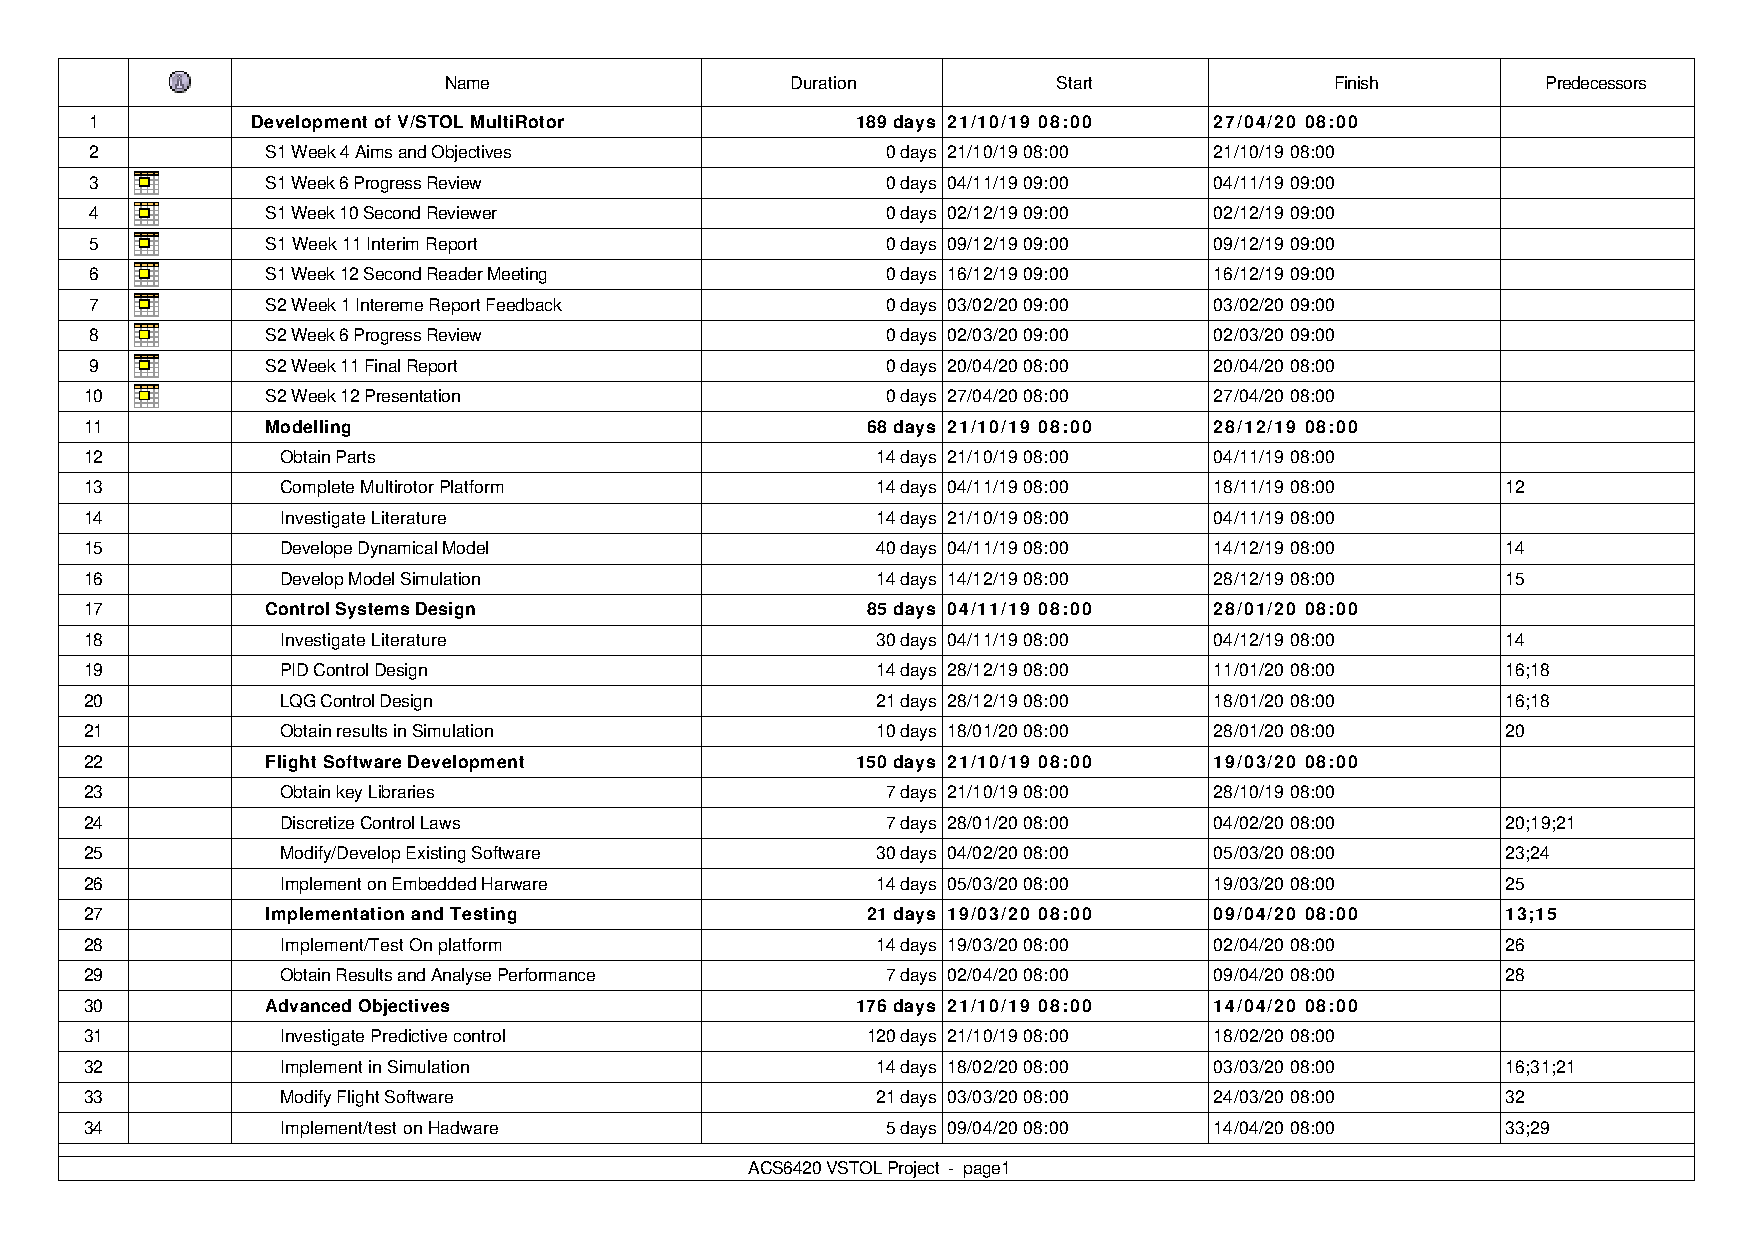
\includepdf[pages=1,pagecommand={},offset=0cm 0cm]{Gantt}
				\caption{Gantt Table of Project Objectives and Dates}
				\label{fig:Gantt Objectives and Dates}
			\end{figure}
		
			\newpage
			
			\begin{figure}[h!]
				\centering 
				\includepdf[pages=2,pagecommand={},offset=0cm 0cm]{Gantt}
				\caption{Gantt Chart Page 1}
				\label{fig:Gantt Chart Page 1}
			\end{figure}
		
			\newpage
			
			\begin{figure}[h!]
				\centering 
				\includepdf[pages=3,pagecommand={},offset=0cm 0cm]{Gantt}
				\caption{Gantt Chart Page 2}
				\label{fig:Gantt Chart Page 2}
			\end{figure}
		
			\newpage
			
			\begin{figure}[h!]
				\centering 
				\includepdf[pages=4,pagecommand={},offset=0cm 0cm]{Gantt}
				\caption{Gantt Chart Page 3}
				\label{fig:Gantt Chart Page 3}
			\end{figure}
		
	\end{appendix}
	
\end{document}